In this chapter, you will learn how to make
free-standing wheat sourdough bread.

\begin{figure}[!htb]
  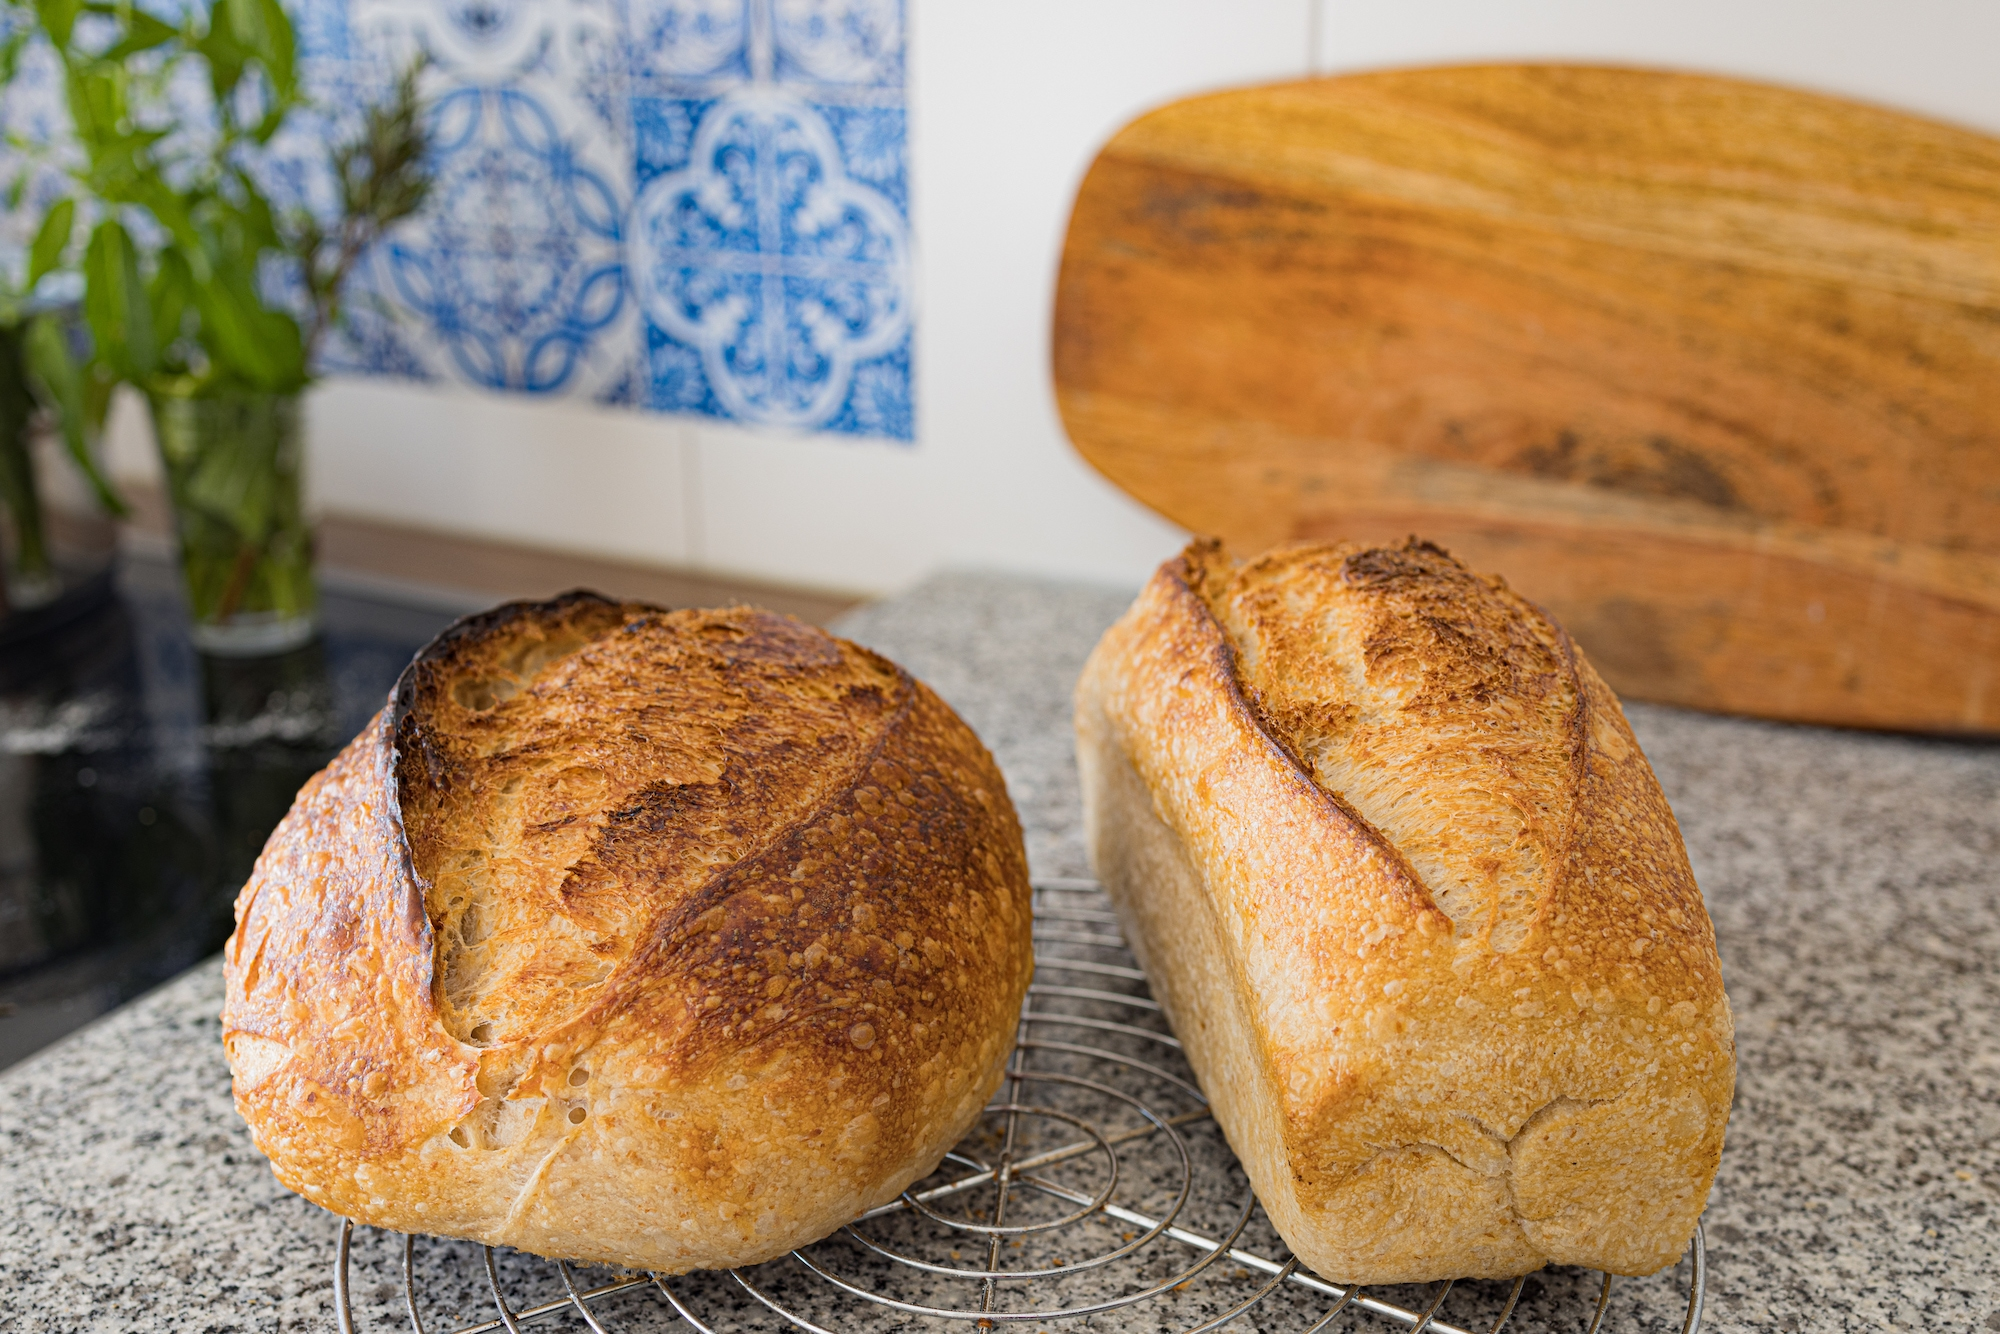
\includegraphics[width=\textwidth]{loaf-pan-free-standing.jpg}
  \caption{A free-standing sourdough bread next to a bread made in a loaf pan.
  The free-standing sourdough is considered the supreme discipline of sourdough bread by many bakers.
  }
\end{figure}

A free-standing sourdough bread is my favorite
type of bread. It combines a great crunchy crust, superb
flavor, and a soft fluffy crumb. This is the type of bread
that is being inhaled by my friends and family. Unfortunately
making this type of bread requires a lot more effort, patience,
and technique than other types of bread. You have to perfectly
balance the fermentation process. You can not ferment for too
short and also not for too long. The techniques you need to
learn require a bit more skill. It took me several attempts
to get this right. One of the challenges I faced was that
I had the wrong flour. I didn't properly know how to use my oven.
When should I stop the fermentation? There is a lot of information
out there. I dug through most of it and have tried almost everything.
In many cases the information was wrong, in other cases, I
found another valuable puzzle piece. Aggregating all this
information was one of my main motivations to start the bread code.
My key learning was that there there is no recipe that
you can blindly follow. You will always have to adapt the recipe
to your local available tools and environment. 

But do not worry. After reading this chapter you will know
all the signs to look out for. You will be able to read your dough.
You will turn into a confident hobby baker that can bake bread
at home, at high altitudes, at low altitudes, in summer, in winter,
at your friend's place, and even on vacation. Furthermore,
you will know how to scale your production from 1 bread to 100 loaves of bread.
If you ever wanted to open up a bakery, consider this knowledge to
be your foundation.

Mastering this process will enable you to make amazing bread
that tastes much better than any store bought bread.

\section{The process}

\begin{figure}[!htb]
  \begin{tikzpicture}[node distance = 3cm, auto]
    \node [block] (init) {\footnotesize Ready starter}; 
    \node [block, right of=init, node distance=3cm] (mix_ingredients) {\footnotesize Mix ingredients}; 
    \node [block, right of=mix_ingredients, node distance=3cm] (dough_strength) {\footnotesize Create dough strength}; 
    \node [block, right of=dough_strength, node distance=3cm] (bulk) {\footnotesize Bulk ferment}; 
    \node [decision, below of=dough_strength, node distance=3cm] (divide_test) {\footnotesize Making 1 loaf?};
    \node [block, left of=divide_test, node distance=3cm] (divide) {\footnotesize Divide}; 
    \node [block, left of=divide, node distance=3cm] (preshape) {\footnotesize Preshape}; 
    \node [block, below of=preshape, node distance=3cm] (shape) {\footnotesize Shape}; 
    \node [block, right of=shape, node distance=3cm] (proof) {\footnotesize Proof}; 
    \node [block, right of=proof, node distance=3cm] (bake) {\footnotesize Bake}; 
    \path [line] (init) -- (mix_ingredients);
    \path [line] (mix_ingredients) -- (dough_strength);
    \path [line] (dough_strength) -- (bulk);
    \path [line] (bulk) -- (divide_test);
    \path [line] (divide_test) -- node{yes} (shape);
    \path [line] (divide_test) -- node{no} (divide);
    \path [line] (divide) -- (preshape);
    \path [line] (preshape) -- (shape);
    \path [line] (shape) -- (proof);
    \path [line] (proof) -- (bake);
  \end{tikzpicture}
  \caption{The typical process of making a wheat based sourdough bread}
  \label{j:wheat-sourdough-process}
\end{figure}

The whole process of making great sourdough bread starts with
readying your sourdough starter. The key to mastering
this process is to manage the fermentation process properly.
For this, the basis is to have an active and healthy
sourdough starter.

Once your starter is ready you proceed to mix all the ingredients.
You want to homogenize your sourdough starter properly. This
way you ensure an even fermentation across your whole dough.

After a short break, you will proceed and create dough strength.
Kneading will create a strong gluten network. This is essential
to properly trap the CO2 created during the fermentation.

Once you kneaded the bulk fermentation starts. Bulk fermentation
because you typically ferment multiple doughs together in one bulk.
Understanding when to stop this step will take some practice.
But nothing to worry about, you will learn the exact signs to look out for.

Once this is completed you need to divide your large blob of
dough into smaller pieces and preshape each piece. This allows
you to apply more dough strength and shape more uniform loaves.

The proofing stage follows where you finish the fermentation process.
Depending on your time you can proof at room temperature or in the fridge.
Mastering proofing will turn your good loaf into a great loaf.

Lastly, you will finish the whole process by baking. You will learn different
options on how to properly steam your dough. This way your
dough will have a beautiful oven spring. During the second
stage of the baking process, you will finish building your crust.

All the steps rely on each other. You will need to get each of
the steps right to make the perfect bread.

\section{Readying your starter}

The most crucial part of the bread-making process is your starter.
The starter is what starts the fermentation in your main dough.
If your starter is off, then your main dough is also going
to cause trouble during the fermentation. Your starter's
properties are passed on to your main dough. If your starter
doesn't have a good balance of yeast to bacteria, so will your
main dough.

\begin{figure}[!htb]
  \begin{tikzpicture}[node distance = 3cm, auto]
    \node [decision] (init) {\footnotesize Starter last fed within 3 days?};
    \node [block, right of=init, node distance=4cm] (feed_no_branch)
      {\footnotesize Feed starter twice. 48 hours before and 6-12 hours before}; 
    \node [block, below of=feed_no_branch, node distance=3cm] (feed_yes_branch)
      {\footnotesize Feed starter once 6-12 hours before making dough}; 
    \node [block, right of=feed_no_branch, node distance=6cm] (high_ratio)
      {\footnotesize Use a 1:10:10 ratio. 10g starter, 100g flour, 100g water}; 
    \node [block, right of=feed_yes_branch, node distance=3cm] (low_ratio)
      {\footnotesize Use a 1:5:5 ratio. 10g starter, 50g flour, 50g water}; 
    \node [block, below of=high_ratio, node distance=6cm] (check_starter)
      {\footnotesize Check if starter is ready to be used}; 
    \node [decision, below of=init, node distance=6cm] (size_check)
      {\footnotesize Bubbly? Increased in size?};
    \node [decision, below of=size_check, node distance=5cm] (smell_check)
      {\footnotesize Vinegary or yogurty smell?};
    \node [block, right of=smell_check, node distance=6cm] (make_dough)
      {\footnotesize Prepare dough}; 
    \path [line] (init) -- node{no} (feed_no_branch);
    \path [line] (init) -- node{yes} (feed_yes_branch);
    \path [line] (feed_yes_branch) -- (low_ratio);
    \path [line] (feed_no_branch) -- (high_ratio);
    \path [line] (high_ratio) -- (check_starter);
    \path [line] (low_ratio) -- (check_starter);
    \path [line] (check_starter) -- (size_check);
    \path [line] (size_check) -- node{no} (feed_yes_branch);
    \path [line] (size_check) -- node{yes} (smell_check);
    \path [line] (smell_check) -- node{no} (feed_yes_branch);
    \path [line] (smell_check) -- node{yes} (make_dough);
  \end{tikzpicture}
  \caption{The process to ready and check your sourdough starter when making a wheat based dough. In practice
  I frequently use a stiff sourdough starter. The stiff starter features enhanced yeast activity. In that case you can
  use the same ratios as shown in the chart except the water quantity. The stiff starter has a hydration of 50 to
  60 percent. So you would half the shown water quantities. I.e. if the chart shows 100g water, use 50 to 60g of water
  for your stiff starter.}
  \label{fig:process-starter-wheat-sourdough}
\end{figure}

Generally, think of the dough you are mixing as a big starter with salt.
After mixing all the ingredients you have a green field environment again.
The yeast and bacteria start to fight again to outcompete each other.
There is plenty of food available and they all do their best to win.
Depending on the starter you mix into your dough some of the microorganisms
might have an advantage over the others.

The first option to achieve a good balance is to apply feedings.
If your starter hasn't been fed in a long period the
bacteria dominate. This happens if your starter has been
sitting unused in the fridge for instance. As more and more
acidity piles up the environment is becoming more and more hostile
to the yeast. The lactic acid bacteria tolerate this environment
better. Your dough fermentation would be more towards the
bacterial side with this starter. By applying a couple of
feedings the yeast becomes more active. The older your
starter the more acid resistant the yeast becomes. Initially,
I had to feed my starter 2-3 times to fix the balance. With my
more mature starter, one feeding seems to be enough to balance
the microorganisms.

Some people use a 1:1:1 ratio to refresh the starter. This would
be one part of the old starter (10g for instance), 1 part of flour,
and one part of water. I think this is utter rubbish. As mentioned
your starter is a gigantic dough. You would never a 1:1:1 ratio to
make a dough. You might use a maximum of 20 percent starter to
make a dough. That's why I advocate using a 1:5:5 ratio or a
1:10:10 ratio depending on how ripe your starter is. As I almost
always use a stiffer sourdough starter due to its enhanced
yeast fermentation advantages (see section \ref{section:stiff-starter})
my ratio is never 1:5:5. My ratio would be 1:5:2.5 (1 part old starter,
5 parts flour, 2.5 parts water). If it is very warm where you live
you could opt for the aforementioned 1:10:5 or 1:20:10. This
way you slow down the ripening of your starter. You can use this
trick too to make starter feeding work with your schedule.
If your starter is typically ready in 6 hours but today you need it
ready later, simply increase how much flour/water you feed your starter.
These are all values that you need to experiment with on your own.
Every starter is unique and might behave slightly different.

The second option at your disposal is the starter quantity that
you use to make the dough. As previously stated your starter
regrows inside of your main dough. While I would normally use
10-20 percent of starter based on the flour, sometimes I go
as low as 1 percent starter. This way the microorganisms have
more room to balance out while fermenting the dough. If my sourdough
starter has not been fed in a day I might use 5 percent of sourdough
to make a dough.  If I push this to 2 days without feedings
I lower the starter amount even further. I would opt for the
previously mentioned 1 percent starter. If the food is very scarce
your microorganisms will sporulate. They need to regrow again
from the spores they created. In this hibernation state, it takes
longer for them to become fully active again. I have tried
several times to make dough directly out of a dry starter.
I wasn't successful because the fermentation took too long.
The microorganisms had to regrow from spores and then begin
the fermentation. As explained earlier there is a limit to
fermentation times as your dough naturally breaks down.
Furthermore, you want your microorganisms to outcompete
other pathogens contained in the flour. The less starter
you use the easier it is for them to reproduce. A strong
starter will outcompete other germs. While the method of
reducing the starter works, I recommend option one more.
It will reliably create better bread. Option 2 is typically
what I use when I fed my starter in the morning but didn't
manage to make a dough in the evening. I don't want to feed
my starter again the next morning. I would like to make a dough
directly without waiting and thus use less of the very ripe starter.

Over time you will become more accustomed to your starter
and how it behaves. You will be able to read the signs of its
activity and judge its state.

\section{Ingredients}

All you need to make a great sourdough bread is flour water and salt. You
can of course add additional things to your dough such as seeds. I personally
enjoy the hearty taste of whole wheat. Thus I like to add around 20-30 percent
of whole wheat flour to the mix. You could also make this recipe with 100 percent
whole wheat flour directly. In this case look out for a strong whole wheat
flour that is made from flour with higher protein. If you don't like whole
wheat you can omit the flour from the recipe. Simply replace the listed
quantity with bread flour. One thing to consider about whole wheat
flour is the increased enzymatic activity. By adding some whole wheat
flour you will speed up the whole fermentation process.

Especially when getting started I recommend to use a bread flour which
contains more gluten than all purpose or cake flour. This is essential
when trying to bake a free standing loaf with sourdough.

Find below an example recipe for 1 loaf including baker's math calculation:

\begin{itemize}
  \item 400g of bread flour
  \item 100g of whole wheat flour
  \item \textbf{500g of flour in total}
  \item 300g-450g of room temperature water (60 percent up to 90 percent). More on
this topic in the next chapter.
  \item 50g of stiff sourdough starter (10 percent)
  \item 10g of salt (2 percent)
\end{itemize}

In case you want to make more bread simply increase the quantities based on
how much flour you have. Let's say you have 2000g of flour available. The
recipe would look like this.

\begin{itemize}
  \item 1800g of bread flour
  \item 200g of whole wheat flour
  \item \textbf{2000g of flour, equalling 4 loaves}
  \item 1200g up to 1800g of room temperature water (60 to 90 percent)
  \item 200g of stiff sourdough starter (10 percent)
  \item 40g of salt (2 percent)
\end{itemize}

This is the beauty of baker's math. Simply recalculate the percentages and you
are good to go. If you are unsure about how this works please check out the
full chapter \ref{section:bakers-math} which looks at the topic in detail.

\section{Hydration}

Hydration refers to how much water you use for your flour. When
beginning to make bread I always got this wrong. I followed a recipe from the
internet and my dough never looked like a dough shown in the recipe.
The amount of water your flour requires is not fixed. It depends on the flour
you have.

When a seed gets into contact initially the outer layers soak up the water.
That's why when using whole wheat (still containing these layers) you have to
use a little bit more water.

By forming gluten strands water is absorbed into your dough. The higher the
protein value the more water can be used.

Some bakers like to use a highly hydrated dough to create a fluffier dough.
\footnote{Sometimes it almost feels like a comparison of skill value between bakers. The
more water they can handle, the more skillful the baker.} The reason for this
is the dough's improved extensibility. The wetter the dough the easier it is
for the dough to be stretched. When you pull it, the dough will hold its
shape. In comparison a very stiff (low hydration) dough will maintain its
shape for a longer period of time. To visualize this think of your extensible
dough as a balloon. The stiff dough is a car tire. The yeast has a much harder
time to inflate the care tire compared to the balloon. That's because the
rubber of the car tire is much more elastic. It requires much more force to
inflate the tire. For this reason an extensible dough will inflate more in the
oven. The loaf will be visually bigger and offer an airier more open crumb structure.

While this might sound great, the high hydration causes several side effects.

\begin{enumerate}
  \item Your dough becomes more difficult to handle. Your dough will be stickier
  \item Your dough has to be kneaded for longer in order to build a proper gluten
    network.
  \item During the fermentation your dough might become too extensible and lose
    some of the dough strength. To circumvent this stretch and folds are applied
    compared to a regular dough.
    requiring you to invest a lot more work.
  \item Shaping becomes much more of a hassle as the dough is very sticky.
  \item The dough can stick to the banneton a lot easier while proofing.
  \item If you wait too long during proofing the dough won't have enough strength
    left to pull upwards and stay flat.
  \item Generally the higher the water content the more bacterial fermentation you
    have. Thus a wetter dough will reduce in gluten faster than a stiffer dough.
    This is why you have to start the fermentation with a sourdough starter in
    perfect shape. Bakers use a process called autolyse to shorten the main
    fermentation time to circumvent this.
  \item The crumb in the end might be perceived as somewhat sticky. It still
    contains a lot of water. Personally I love this crumb, but this is a personal
    choice.
\end{enumerate}

To achieve a high hydration dough it is best to slowly add the water to
your dough. Start with 60 percent hydration, then slowly add a bit more water. Knead
again until the water is absorbed. Repeat and add more water. As your dough
has already formed a gluten network, new water can be absorbed much easier.
You will be surprised by how much water your dough can soak up. This
method is commonly known as the bassinage method. More on that later.
By opting for this technique I was easily able to push a low
gluten flour to a hydration of 80 percent. This
is also my method of choice when making a dough now. I keep adding water until
I can feel that the dough has the right consistency. As you bake more bread
you will develop a better look and feel for your dough. When mixing
by hand this can be quite cumbersome. It is a lot more easy when using a stand
mixer.

All in all increasing the hydration requires a lot of trial and error. There
is however one option that makes things easier and causes less headache:
Slow fermentation. You get the same extensibility advantages the high hydration
offers by simply letting your dough ferment for a longer period of time.
Slowing the fermentation process is easy. Use less
sourdough starter or ferment in a cooler environment. 

There are two reasons for slow fermentation advantages.
As explained earlier both the protease enzyme and bacteria break down your
gluten network. So as fermentation progresses your dough will automatically
become more extensible. This is because the rubber layers of your care tire
are slowly converted and eaten. Ultimately your car tire turns into a balloon
that can very easily be inflated.  When waiting too long the
balloon will burst. You will have no gluten left anymore and your dough
becomes very sticky. Finding the sweet spot of enough rubber eating and not
too much is what the perfect wheat sourdough bread bread is about. But don't worry, after reading
this chapter you will have the right tools at your disposal.

The advantages of slow fermentation can be nicely observed when experimenting
with a fast fermenting yeast dough (1 percent dry yeast based on the flour). The
crumb of such a dough is never as
open as a dough made with sourdough. Furthermore the protease enzyme
can not do its job within such a short fermentation period.
Large industrial bakeries add active malt which contains a
lot more enzymes. This way the time required to make a dough is shortened. You
will most likely find malt as an ingredient in supermarket bread. It is a
great hack. The baked turbo fermentation bread will feature a relatively dense
and not fluffy crumb. That is because only very little gluten is broken down when
finishing the fermentation period in 1 hour. If you were to slow down things
the dough would look completely different.
Try this again and use way less yeast. This is the
secret of the Neapolitan Pizza. Only a tiny bit of yeast is used to make the
dough. In fact my default pizza recipe calls for around 150 milligrams of dry
yeast per one kilogram of flour. Give it a shot yourself the next time you
make a yeast based dough. Try to push the fermentation to at least 8 hours.
The difference is incredible. You will have made a bread with a much more
fluffy and open crumb. The flavor of the dough is drastically improved. Your
crust becomes crisper and features a better taste. This is because amylases have
converted your starches into simpler sugars which brown better during baking.
If you take away one learning from this book, it is that slow fermentation is
the key to making great bread.

For this reason my default hydration is much lower than the hydration of other
bakers. I prefer a slower fermentation for my recipes.
The sweet spot for my default flour is at around 70 percent hydration.
Again this is a highly subjective value that works for my flour.

If you are just getting started with a new batch of flour
I recommend to conduct the following test. This will help you to
identify the sweet spot of your flour's hydration capabilities.

Make 5 bowls with each 100g of flour. Add different slightly increasing 
water amounts to each of the bowls.

\begin{itemize}
  \item 100g of flour, 55g of water
  \item 100g of flour, 60g of water
  \item 100g of flour, 65g of water
  \item 100g of flour, 70g of water
  \item 100g of flour, 75g of water
\end{itemize}

Proceed and mix the flour and water mixture until you see that there
are no chunks of flour left. Wait 15 minutes and return to your doughs.
Carefully pull the dough apart with your hands. Your dough should be elastic
and hold together. Stretch your dough until very thin. Then hold it against a light.
You should be able to see through it. The flour water mixture that breaks without
seeing the windowpane is your no-go zone. Opt for a dough with
less hydration than this value. You will know that your flour mix can go up to
65 percent hydration for instance. Use the left overs of this experiment
to feed your starter.


\begin{figure}[!htb]
  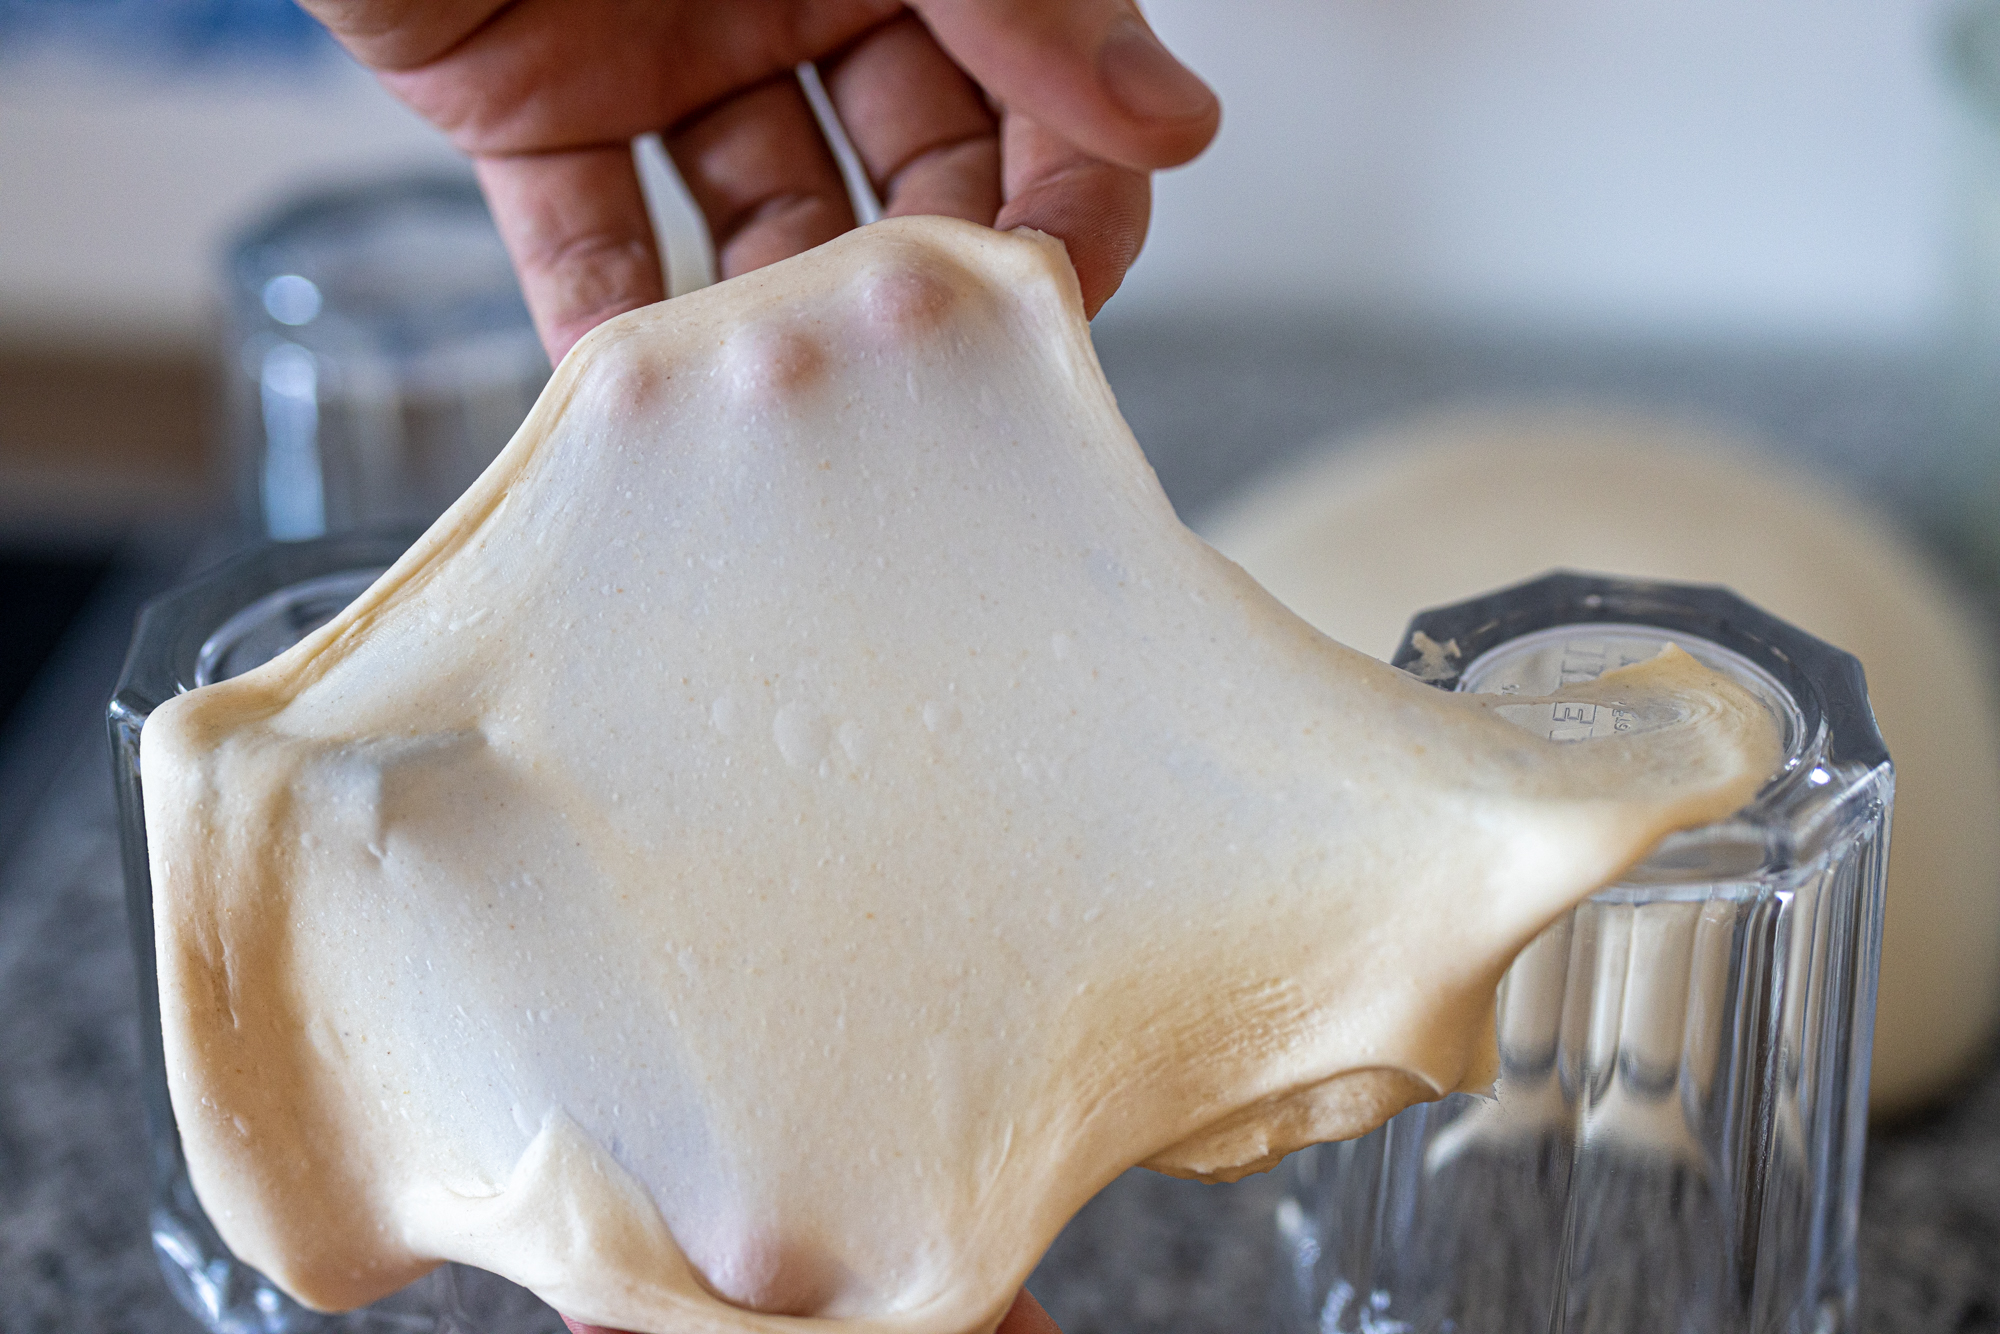
\includegraphics[width=\textwidth]{window-pane-effect}
  \caption
    {The window pane test allows you to see if you developed your gluten well enough}
\end{figure}


From an economic perspective water is the cheapest component in your bread
dough. When running a bakery a higher hydrated dough will weigh more have
lower production costs. The profit will be higher. This comes at the price
of increasing labor costs and more potential failures due to the enhanced
difficulty.

\section{How much starter?}

Most bakers use around 20 percent sourdough starter based on the dough mass. I
recommend to go way lower to around 5 to 10 percent.

By adjusting the amount of preferment you can influence the time your dough
requires in the bulk fermentation stage. The more starter you use the faster
this process is. The smaller the amount of starter the slower. With a higher
quantity of starter you are introducing more microorganisms to your main
dough. The higher this quantity the faster the rate of fermentation in your
dough is.

The other factor influecing the rate of fermentation is the temperature of
your dough. The warmer the temperature the faster the process, the colder the
slower the process.

While food is available the microorganisms will reproduce and increase in
quantity. The process is a self limiting process that stops when there is no
more food available. This can be compared to whine making where
the yeast ultimately dies as ethanol levels increase and turn the environment
toxic. The ethanol creates a preservant that makes it impossible for other
microorganisms to join the feast. The same thing happens with the acidity
created by the bacteria. The high acidity slows the fermentation process and
prevents new microorganisms from entering the system.

Initially your starter's properties are carried over to the main dough. Then
as time progresses the microorganisms adapt to the new environment. If your
starter is very bacterial then so will be your main dough's fermentation. You
end up with a dough that is not as fluffy as it could be. It will taste quite
sour, too sour for most people.

If you were to use an extreme value of around 90 percent starter based on your flour there
would be very little room for the microorganisms to adjust in the main dough.
If you were to just use 1 percent, your microorganisms can regrow into a
desirable balance in the dough. Furthermore you need to consider that a high value
of starter means a high inoculation with already fermented flour. As
mentioned earlier enzymes break down the dough. This means the higher this
value the more broken down fermented flour you have. A too long fermentation
always results in a very sticky dough that can not be handled. The more
starter you use the faster you will get to this point. If you were to use a
very little amount of starter your flour might have naturally broken down
before the fermentation has reached the desired stage. You can observe this
when using a small quantity of around 1 percent sourdough starter. The small
amount of added microorganisms will not be able to reproduce fast enough
before the protease has broken down your dough completely.

As explained earlier the key to making great bread is a slow but not too slow
fermentation. Enzymes require time to break down your dough. Taking all this
into consideration I try to aim for a fermentation time of around 8 to 12 hours. This seems to be
the sweet spot for most of the flours that I have worked with. To achieve this
I use around 5 percent of sourdough starter in summer times (temperatures are
at around 25°C in the kitchen.). In winter times I opt for around 10 percent
up to 20 percent sourdough starter (kitchen temperature around 20°C). This
allows me to use a sourdough starter that's not in perfect condition. Your
bread dough is essentially a gigantic starter. The low inoculation rate allows
the starter to regrow inside of your main dough into a desirable balance.
Furthermore the enzymes have enough time to break down the flour. This also
allows me to skip the so called autolysis step completely (more in next chapter).
 Making a dough becomes very simple.

\section{Autolyse}

The autolysis describes the process of just mixing flour and water and letting
this sit for a period of around 30 minutes up to several hours. After this
process is completed the sourdough starter and salt is added to the
dough.\footnote{I have tested adding the salt at the start and end of the
autolysis process and could not notice a difference. Based ony my current
understanding the importance of adding salt later seems to be a myth.}

The overall time flour and water is in contact is extended. Thus you get the
beneficial enzymatic reactions that improve taste and characteristics of the
dough. I do not recommend an autolysis as it adds an additional step in the
process. Instead I recommend the fermentolyse which will be covered in the
next chapter of this book.

The effects of the autolysis are very interesting. Try to mix just flour and
water and letting that sit for a day. During the day check the consistency of
your dough. Try and stretch the dough. If you dare you can also taste the
dough throughout the day. With each hour progressing your dough will become
more extensible. It will be easier to stretch the dough. At the same time your
dough will start to taste sweet and sweeter. The protease and amylase enzymes
are doing their job. The same process is used when making oat milk. By letting
the mixture sit for some time enzymes work the oats. The taste is perceived as
sweeter and more appreciated. This process is further accelerated the more
whole wheat your flour is. The hull contains more enzymes. The gluten network
will ultimately tear and your dough flattens out. For wheat sourdough this is
your worst enemy. When this happen your dough will become leaky and release
all that precious gas created during the fermentation. You need to find the
right balance of your dough breaking down just enough and not too much.

When you use a high inoculation rate of around 20 percent sourdough starter
your fermentation can be very quick. At 25°C it could be finished in 5 hours
already. If you ferment longer your dough becomes leaky. At the same time in
these 5 hours the enzymes have not broken down the flour enough. This means
the dough might not be as elastic as it should be. Furthermore not enough
sugars have been released and thus the flavor after baking is not good enough.
\footnote{I have not seen studies yet looking at enzymatic speeds depending on
the temperature. But I assume the higher the temperature the faster these
reactions. This goes up until to a point when the enzymes break down under
heat.} That's why bakers opt for the autolyse. The autolyse starts the enzymatic
reactions before the microorganism fermentation begins. This way after 2 hours
of autolysis (an example) and 5 hours of fermentation the dough is in the
perfect state before beginning proofing.

When you try to mix your salt and starter into the flour/water dough you will
notice how cumbersome this is. It feels like you have to knead again from scratch
one more time. You will spend more time on mixing a dough.

For that reason I am advocating to utilize the fermentolyse which simplifies
the mixing and kneading process greatly.

\section{Fermentolyse}

The fermentolyse creates you the same advantageous dough properties the
autolysis creates without the headache of mixing your dough twice. You do this
by extending the fermentation time of your dough. Rather than doing a 2 hour
autolysis and 5 hour bulk fermentation you opt for an overall 7 hour
fermentation period.

To do this you use less sourdough starter. A conventional recipe including the
autolysis step might call for 20 percent sourdough starter. Simply reduce this
value to 5-10 percent. The other option could be to place the dough in a colder
environment and thus reduce the speed at which your microorganisms replicate.

\begin{table}[!htb]
  \begin{tabular}{|l|l|l|l|}
  \hline
  \textbf{\begin{tabular}[c]{@{}l@{}}Temperature\\ in °C\end{tabular}} & \textbf{\begin{tabular}[c]{@{}l@{}}Temperature\\ in °F\end{tabular}} & \textbf{\begin{tabular}[c]{@{}l@{}}Starter\\ recently fed?\end{tabular}} & \textbf{\begin{tabular}[c]{@{}l@{}}Amount\\ of starter in\%\end{tabular}} \\ \hline
  30                                                                   & 86                                                                   & Yes                                                                      & 5                                                                         \\ \hline
  25                                                                   & 77                                                                   & Yes                                                                      & 10                                                                        \\ \hline
  20                                                                   & 68                                                                   & Yes                                                                      & 15                                                                        \\ \hline
  30                                                                   & 86                                                                   & No                                                                       & 2.5                                                                       \\ \hline
  25                                                                   & 77                                                                   & No                                                                       & 5                                                                         \\ \hline
  20                                                                   & 68                                                                   & No                                                                       & 10                                                                        \\ \hline
  \end{tabular}
  \caption{A table visualizing how much sourdough starter to use depending on temperature and the starter's activity level}
\end{table}

Based on my experience and my sourdough my ideal breads always take around 8
to 12 hours during the bulk fermentation. Based on my availability throughout
the day I use more or less starter. If I wanted to achieve a completed
fermentation in 8 hours I would opt for 10 percent sourdough starter. If I
wanted it to be ready in 12 hours I would use less starter, around 5 percent.
Simply mix together all the ingredients and your fermentation begins. The
enzymes and microorganisms commence their work. On a very warm summer day the
mentioned quantities no longer work. With 10 percent starter the same dough
would be ready in 5 hours up to a point of no return. Another additional hour
would cause the dough to break down too much. In this case I would opt for 5
percent sourdough starter to slow the whole process down to reach the 8 to 12
hour window again. If it is very hot I might use as little as 1 percent
sourdough starter.\footnote{Please take these values with a grain of salt as
they depend on your flour and your sourdough starter. These are values that
you have to experiment with. After baking a couple of breads you will be able
to read your dough much better.} You have to play with the timings on your own.
Rather than relying on timing I will show you a much better and more precise approach
by using a fermentation sample. This will be covered later in this chapter.

Even for yeasted doughs I no longer use an autolysis. I just reduce the amount
of yeast that I am using. Opting for the fermentolysis will
save you time and simplify your bread making. As mentioned in previous chapters,
the secret to making great bread is a slow but not too slow fermentation.

\section{Dough strength}

Dough strength is a fancy way to describe the bread kneading process. As you wait and
knead the gluten bonds in your dough become stronger. The dough
becomes more elastic and holds together better. This is the basis for trapping
all the gases during the fermentation process. Without the gluten network
the gases would just diffuse out of your dough.

\begin{figure}[!htb]
  \begin{tikzpicture}[node distance = 3cm, auto]
    \node [block] (init) {\footnotesize Homogenize recipe ingredients}; 
    \node [block, right of=init, node distance=3cm] (wait1) {\footnotesize Wait 15 minutes};
    \path [line] (init) -- (wait1);
    \node [block, right of=wait1, node distance=3cm] (knead1) {\footnotesize Knead 5 minutes};
    \path [line] (wait1) -- (knead1);
    \node [block, right of=knead1, node distance=3cm] (wait2) {\footnotesize Wait 15 minutes};
    \path [line] (knead1) -- (wait2);
    \node [decision, below of=wait2, node distance=3cm] (windowpane_test) {\footnotesize Window-pane?};
      \path [line] (wait2) -- (windowpane_test);
      \path [line] (windowpane_test) -- node{no} (knead1);
    \node [decision, left of=windowpane_test, node distance=4.5cm] (more_water) {\footnotesize Bassinage for more water?};
      \path [line] (windowpane_test) -- node{yes} (more_water);
    \node [block, left of=more_water, node distance=4.5cm] (add_water) {\footnotesize Add water};
      \path [line] (more_water) -- node{yes} (add_water);
      \path [line] (add_water) -- (knead1);
    \node [block, below of=add_water, node distance=4cm] (wait3) {\footnotesize Wait 15 minutes};
    \path [line] (add_water) -- (wait3);
    \node [decision, right of=wait3, node distance=4.5cm] (dough_sample) {\footnotesize Aliquot jar?};
    \path [line] (wait3) -- (dough_sample);
    \path [line] (more_water) -- node{no} (dough_sample);
    \node [block, right of=dough_sample, node distance=4.5cm] (dough_ball) {\footnotesize Make round dough ball};
    \path [line] (dough_sample) -- node{no} (dough_ball);
    \node [block, below of=dough_sample, node distance=3cm] (extract_sample) {\footnotesize Extract sample};
    \path [line] (dough_sample) -- node{yes} (extract_sample);
    \path [line] (extract_sample) -- (dough_ball);
    \node [block, below of=dough_ball, node distance=3cm] (begin_bulk) {\footnotesize Begin bulk fermentation};
    \path [line] (dough_ball) -- (begin_bulk);
  \end{tikzpicture}
  \caption{The gluten development process for a wheat based dough}
  \label{fig:wheat-sourdough-kneading-process}
\end{figure}

It might sound odd but the most important part of kneading is waiting. By
waiting you are allowing your flour to soak up water. This way the gluten
bonds of your dough form automatically and your dough becomes more elastic.
So you could be kneading for 10 minutes initially just to be surprised
that kneading 5 minutes and waiting 15 minutes has the same effect.

The gluten proteins glutenin and gliadin virtually instantly bond after being
hydrated. Disulfide bonds enable the longer portions of
glutenin to join with one another and form sturdy, extensible molecules.
Glutenins add strength, whilst the more compact gliadin proteins allow
the dough to flow like a fluid. Ultimately the longer you wait, the more
your gluten network transforms into a web like structure. This is what
traps the gases during the fermentation process. \cite{how+does+gluten+work}.

\begin{figure}[!htb]
  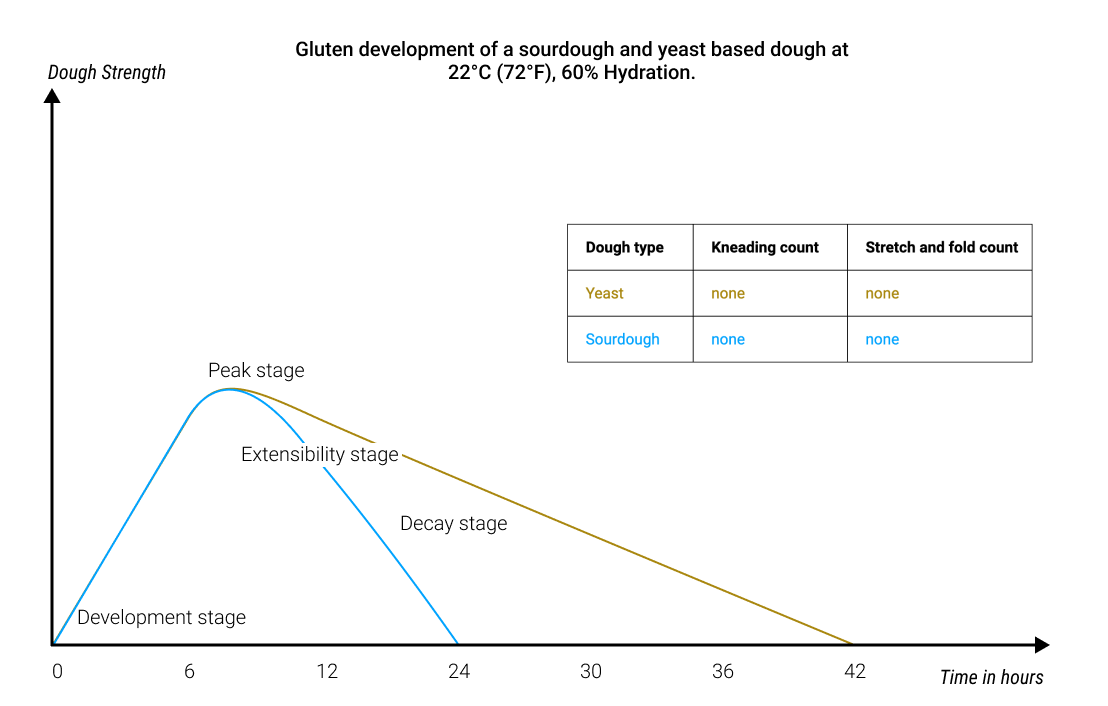
\includegraphics[width=\textwidth]{dough-strength-sourdough-yeast}
  \caption{A schematic visualization of
  automatic gluten development. The doughs are not kneaded, just initially
  mixed. Note how the dough strength
  deteriorates over time as enzymes break down the flour. The effect
  is accelerated for sourdough due to the bacteria's gluten proteolysis.
  }
  \label{fig:wheat-yeast-sourdough-degradation}
\end{figure}
% See https://www.figma.com/file/wTUVe6Nm2INOvT82mJhQur/Dough-strength-visualisation?node-id=0%3A1&t=fjdPvXYuJpsdQfWN-1 for
% the source of this visualization

The soaking process has to be extended the more whole wheat flour is used.
The purpose of the wheat kernel's outer bran is to soak up water as fast
as possible. The enzymes become activated and start the sprouting process.
Because of this less water is available for the gluten bonds to develop.
Either wait a bit longer, or proceed and use slightly more water for
the dough.

This is the same principle that popular no-knead recipes follow. By making a less
hydrated dough and waiting your gluten network automatically forms. You still
have to mix and homogenize the ingredients. You wait a few minutes just to
find your dough having developed incredible dough strength with no additional
kneading.\footnote{Give it a shot yourself. The automatic formation of gluten
networks is an amazing phenomenon that still fascinates me every time I am
making a dough.}

If you over hydrate your dough at the beginning it becomes more difficult
for the gluten chains to form. The molecules are not as close together in
a wetter dough compared to a stiffer dough. It is harder for the molecules
to align and form the web structure. For this reason it is always easier
to start with a lower hydration and then increase the water quantity if needed.
This is also commonly known as the \textit{Bassinage method}. The gluten
bonds have formed at the lower hydration and can then be made more extensible
by adding water and kneading again. This is a great trick to make
a more extensible dough with a lower gluten flour. \cite{bassinage+technique}

When machine kneading a dough opt for the same technique shown in figure \ref*{fig:wheat-sourdough-kneading-process}.
Initially opt for a low speed. This helps the homogenization process.
After waiting to allow the flour to soak up the water, proceed on a higher speed
setting. A good sign of a well developed gluten network is
that your dough lets go of the container. This is because the gluten's elasticity.
The elasticity is higher than the urge of the
dough to stick to the container. 

\begin{figure}[!htb]
  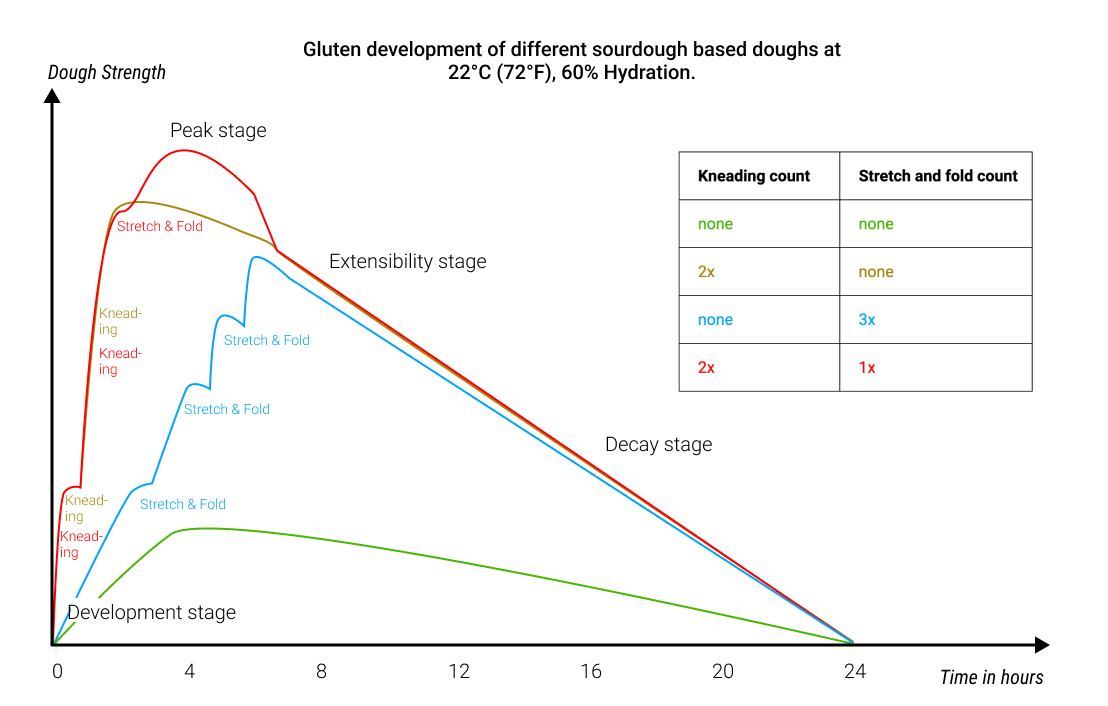
\includegraphics[width=\textwidth]{dough-strength-sourdough}
  \caption{A schematic visualization of
  gluten development in sourdoughs with different kneading techniques.
  A combination of techniques can be utilized to achieve maximum
  dough strength.
  }
\end{figure}
% See https://www.figma.com/file/wTUVe6Nm2INOvT82mJhQur/Dough-strength-visualisation?node-id=0%3A1&t=fjdPvXYuJpsdQfWN-1 for
% the source of this visualization

Generally the more dough strength you create, the less sticky your dough is going to
feel. As the dough holds together it will no longer stick to your hands as
much. This is a common problem beginners face. A sticky dough is frequently
the sign of a not well enough developed gluten network.

\begin{figure}[!htb]
  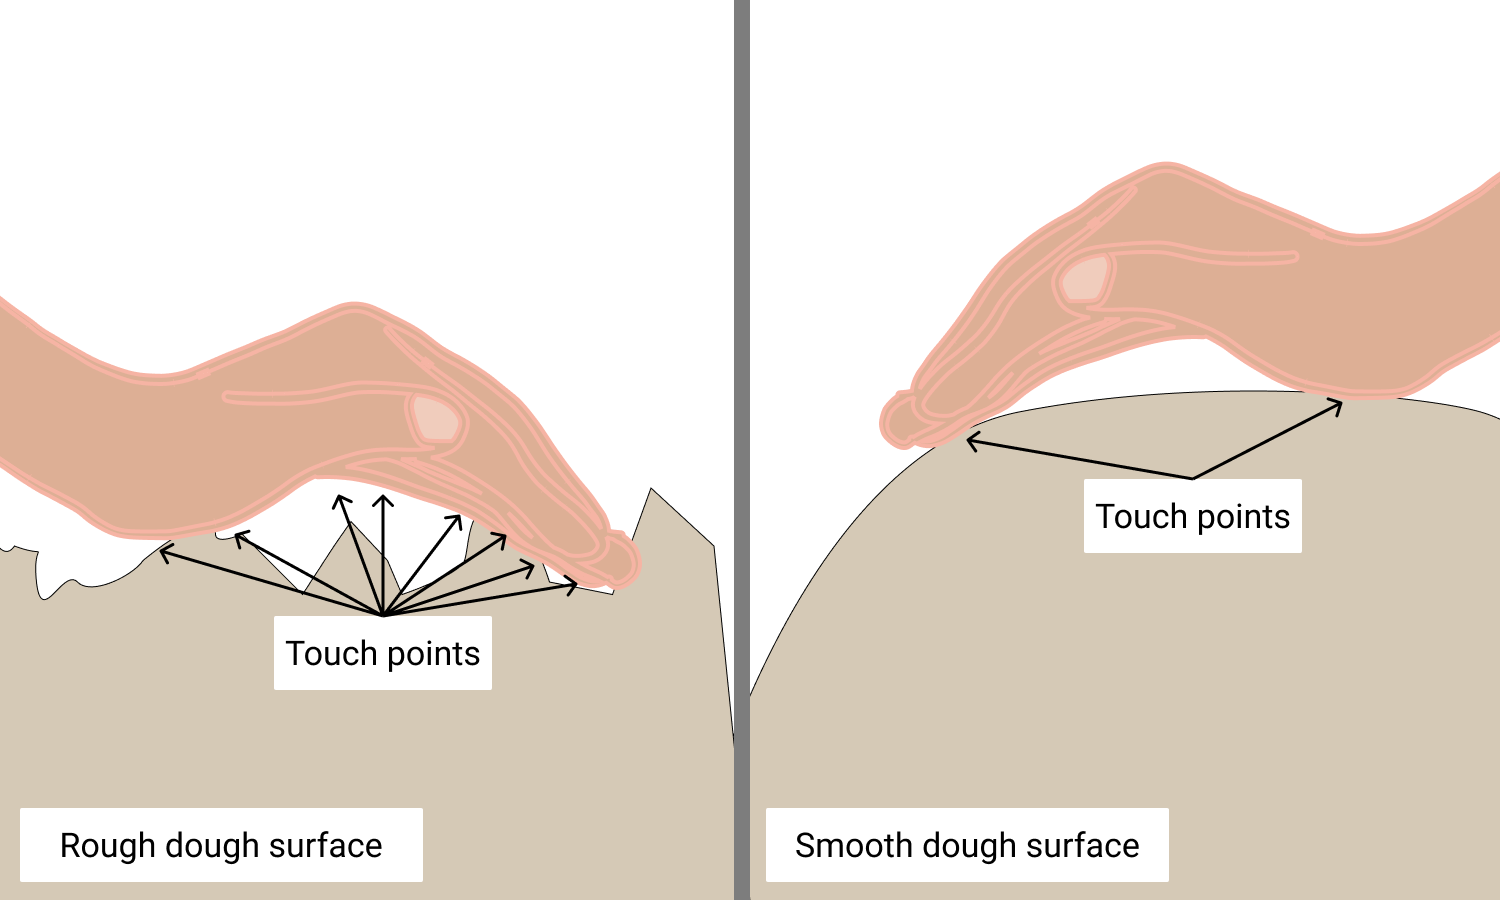
\includegraphics[width=\textwidth]{dough-surface-touchpoints}
  \caption{A schematic visualization of how a rough dough surface
  creates more touch points compared to a smooth dough surface.
  By touching the rough surface the dough will swell and get into
  contact with more areas of your hand.
  }
  \label{fig:dough-touch-points}
\end{figure}

Kneading more is great in almost all cases. You'll have a stronger
gluten network. Only in case you are making soft milk breads you
might want to have a more extensible dough to begin with. For every
other type of wheat based dough kneading is helpful. When you use
a stand mixer, you can run into the issue of kneading too much. This
is hardly possible though. Even after kneading for 30 minutes on medium
speed my doughs hardly ever were over-kneaded. The moment you knead
too much the color of the dough can begin to change. You mostly
notice this though during baking. The resulting loaf looks very
pale and white. This is because mixing dough causes oxidation,
which is necessary for the development of gluten.
However, if the dough is mixed too much, the compounds that contribute
to the bread's flavor, aroma, and color may be destroyed, negatively
affecting the quality of the bread.\cite{oxidization+dough}

The last step before beginning bulk fermentation is to
create a smooth dough ball. By making sure your dough's surface is
smooth you will have fewer touch points when touching the dough.
See figure \ref{fig:dough-touch-points} for a schematic visualization
of how your hand touches a rugged and smooth dough.
With the smooth surface your dough is going to stick less on your hands. Applying
later stretch and folds will be a lot easier. Without a smooth
surface, the dough becomes almost unworkable. Folding the dough later
becomes an impossible task. This is a frequent mistake I see many
new bakers commit.

\begin{figure}[!htb]
  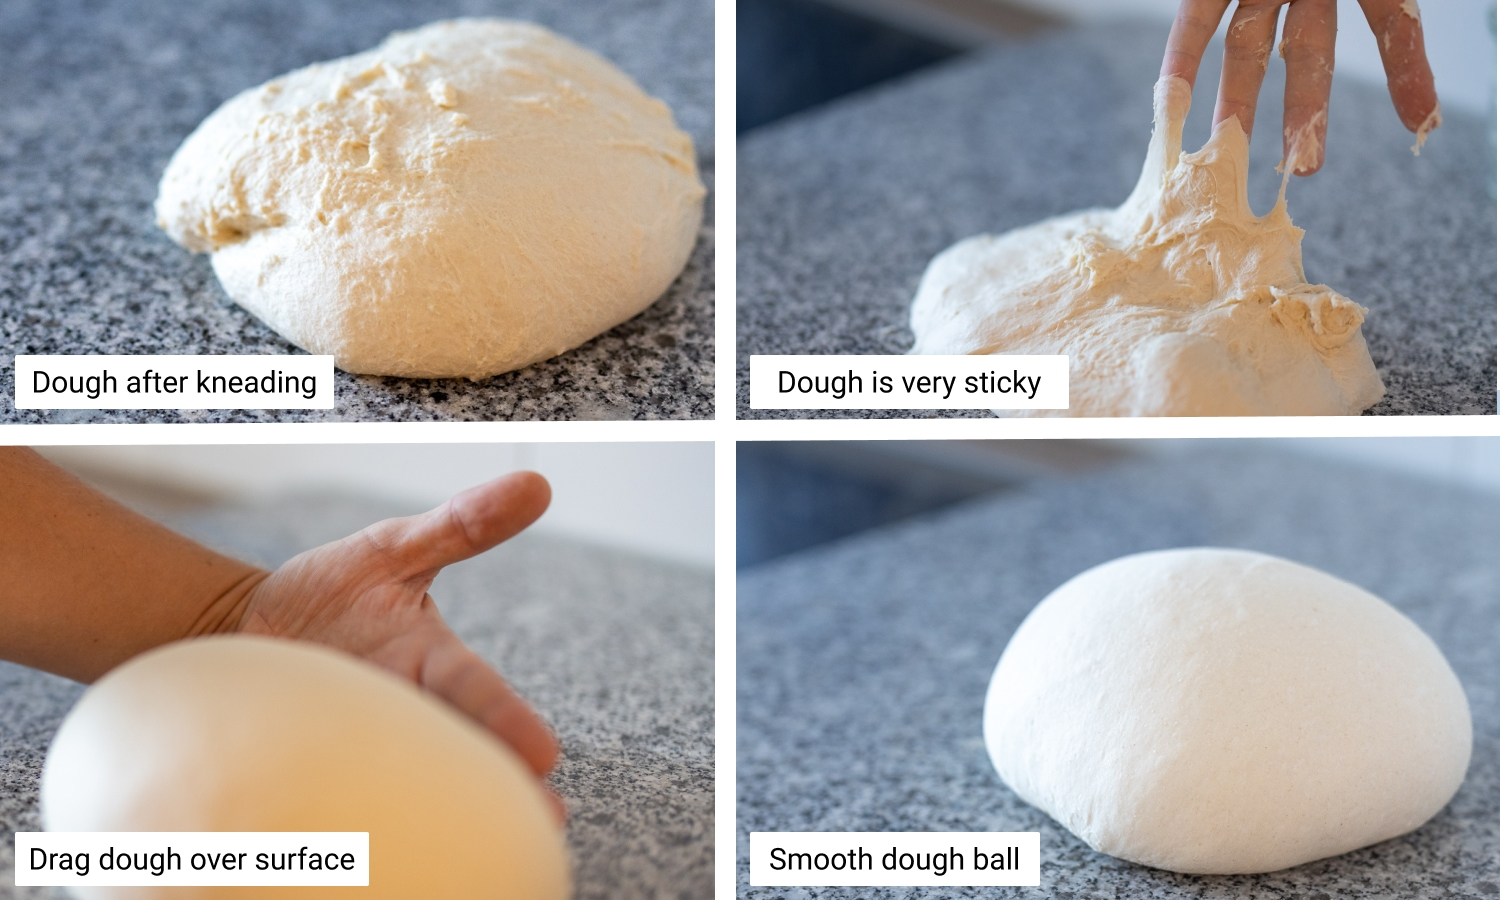
\includegraphics[width=\textwidth]{dough-ball-steps}
  \caption{The transformation of a sticky dough blob to a dough
  with a smooth surface. The goal is to reduce surface touchpoints
  with your hands to make the dough less sticky when working it.
  }
  \label{fig:dough-ball-steps}
\end{figure}


To make the dough's surface smooth place your dough on a wooden board or
on your kitchen's countertop. Drag the dough with your palm over the surface.
A dough scraper could be used here for assistance.
Drag the dough towards you while making sure the top center of the dough stays in place.
It can help to gently place your second hand on top of the dough so that
the dough mass moves while retaining its orientation. Once the whole dough
is too close to the edge of the container/countertop gently move it back
with two hands. By doing so you are stretching the outer surrounding gluten layer.
For this reason, it is important to not use any flour during this process.
By using flour you can no longer drag the dough over the surface and thus
you can't stretch the gluten. Always imagine you are touching something utterly sticky.
By doing so you will automatically try to touch the dough as little
as possible. Keep repeating the process until you see that the dough
has a nice smooth surface. The final dough should look like the dough
shown in \ref{fig:dough-ball-steps}.

If your outer gluten layer tears you have overstretched your dough. In
that case, take a 10-minute break leaving your dough on the kitchen countertop. 
This allows the gluten to re-bond and heal. Repeat the same process
and the damaged rugged areas should disappear.

The same dough-rounding technique is used later during
the pre-shaping process. After creating dough strength you
have all the time you need to practice rounding. Round the dough
as much as possible until it tears. Then wait the mentioned 10 minutes and repeat.
Later you don't have any room for error. Your technique has to be on point.
An over-pre-shaped dough can potentially not recover.


\section{Bulk fermentation}

After mixing the starter into your dough the next stage of
the process known as bulk fermentation begins. The term
bulk is used because in bakeries multiple loaves are fermented
together in bulk. If you are a home baker you might bulk
ferment a single loaf. The bulk fermentation ends when you
divide and preshape, or directly shape your final loaves or loaf.

The hardest part when making sourdough bread is controlling
the fermentation process. Bulking long enough but not too
long is the deciding factor for making great bread at home.
Even with poor shaping and baking techniques, you'll be able
to make excellent bread, solely by mastering the bulk
fermentation process.

With a too-short bulk, your crumb will be
perceived as gummy. Your crumb will feature large pockets of
air commonly referred to as "craters". A too-long fermentation
results in the dough breaking down too much. The resulting
dough will stick to your banneton and spread while baking
into a pancake-like structure.

The key is to find the sweet spot between not too little
and not too much bulk fermentation. I'd always recommend pushing
the dough more toward a longer fermentation. The
flavor of the resulting bread is better compared to a pale
underfermented dough. 

\begin{table}[!htb]
  \small
  \begin{tabular}{|l|l|l|l|}
  \hline
  \textbf{}                                                        & \textbf{\begin{tabular}[c]{@{}l@{}}Too short\\ fermentation\end{tabular}}                                                   & \textbf{\begin{tabular}[c]{@{}l@{}}Too long\\ fermentation\end{tabular}}                                    & \textbf{\begin{tabular}[c]{@{}l@{}}Perfect\\ fermentation\end{tabular}}                                                                                    \\ \hline
  \textbf{\begin{tabular}[c]{@{}l@{}}Crumb\\ texture\end{tabular}} & \begin{tabular}[c]{@{}l@{}}Unbaked gummy areas\\ towards the bottom of\\ the bread\end{tabular}                             & \begin{tabular}[c]{@{}l@{}}Crumb can be\\ perceived as\\ gummy, as most\\ gluten broken\\ down\end{tabular} & \begin{tabular}[c]{@{}l@{}}Crumb evenly baked.\\ Crumb can be perceived\\ as moist, but not\\ gummy\end{tabular}                                           \\ \hline
  \textbf{Alveoli}                                                 & \begin{tabular}[c]{@{}l@{}}Overly large alveoli\\ in the crumb "craters"\end{tabular}                                       & \begin{tabular}[c]{@{}l@{}}Many tiny alveoli\\ equally distributed\end{tabular}                             & \begin{tabular}[c]{@{}l@{}}Alveoli evenly\\ distributed, no\\ "craters"\end{tabular}                                                                       \\ \hline
  \textbf{Taste}                                                   & Pale neutral taste                                                                                                          & \begin{tabular}[c]{@{}l@{}}Strong acidic flavor\\ profile. Acidity\\ overweighs when\\ tasting\end{tabular} & \begin{tabular}[c]{@{}l@{}}Balanced flavor profile,\\ not too mild but also\\ not too sour. Depending\\ on starter vinegary\\ or lactic notes\end{tabular} \\ \hline
  \textbf{Texture}                                                 & Overall poor Texture                                                                                                        & \begin{tabular}[c]{@{}l@{}}Good consistency,\\ crumb is not as fluffy\\ as it could be\end{tabular}         & \begin{tabular}[c]{@{}l@{}}Great combination of \\ textures\end{tabular}                                                                                   \\ \hline
  \textbf{\begin{tabular}[c]{@{}l@{}}Oven\\ spring\end{tabular}}   & \begin{tabular}[c]{@{}l@{}}Vertical oven spring,\\ mostly due to water\\ evaporating and\\ inflating the dough\end{tabular} & \begin{tabular}[c]{@{}l@{}}Very flat pancake like \\ structure after baking\end{tabular}                    & \begin{tabular}[c]{@{}l@{}}Great vertical oven\\ spring. Dough grows\\ more upwards rather\\ than sideways\end{tabular}                                    \\ \hline
  \end{tabular}
  \caption{The different stages of sourdough fermentation and the effects on crumb, alveoli, texture, and overall taste.}
\end{table}

The worst thing you can do when fermenting sourdough 
is to rely on a recipe's timing suggestions. In 99 percent
of the cases, the timing will not work for you. The writer
of the recipe probably has different flour and a different
sourdough starter with different levels of activity. Furthermore,
the temperature of the fermentation environment might be
different. Just small changes in one parameter result
in a completely different timing schedule. One or two hours
difference results in the dough not fermenting long enough, or
turning it into a gigantic sticky fermented pancake. This
is one of the reasons why the current baking industry prefers
to make solely yeast-based doughs. By removing the bacteria
from the fermentation, the whole process becomes a lot more
predictable. The room for error (as shown in figure \ref{fig:wheat-yeast-sourdough-degradation})
is much larger. The doughs are perfect to be made in a
machine.

Experienced bakers will tell you to go by the look and feel of
the dough. While this works if you have made hundreds of loaves,
this is not an option for an inexperienced baker. As
you make more and more dough you will be able to judge
the dough's state by touching it. 

My go-to method for beginners is to use an \textbf{Aliquot jar}.
The aliquot is a sample that you extract from your dough. The
sample is extracted after creating the initial dough strength.
You monitor the aliquot's size increase to judge the
level of fermentation of your main dough. The aliquot
jar is extracted after creating dough strength. As your
dough ferments, so does the content of your aliquot jar. The moment your
sample reached a certain size your main dough is ready
to be shaped and proofed. The size increase you should
aim for depends on the flour you have at hand. A flour
with a higher gluten content can be fermented for a
longer period. Generally, around 80 percent
of your wheat flour's protein is gluten. Check your flour's
packaging to see the protein percentage. The actual size increase
value is highly subjective depending on your flour composition.
I recommend beginning with a size increase of 25 percent and testing
up to 100 percent with subsequent bakes. Then identify a value
that you are happy with.

\begin{table}[!htb]
  \begin{tabular}{|r|r|}
  \hline
  \multicolumn{1}{|l|}{\textbf{Flour protein content}} & \multicolumn{1}{l|}{\textbf{Relative aliquot size increase}} \\ \hline
  8-10\%                                               & 25\%                                                         \\ \hline
  10-12\%                                              & 50\%                                                         \\ \hline
  12-15\%                                              & 100\%                                                        \\ \hline
  \textgreater 15\%                                    & \textgreater 100\%                                           \\ \hline
  \end{tabular}
  \caption{Reference values for how much size increase to aim for with an aliquot jar depending on the dough's protein content}
\end{table}

The beauty of the aliquot is that no matter the surrounding
temperature, you will always know when your dough is ready.
While the dough might be ready in 8 hours in summer, it could
easily be 12 hours in winter. You will always ferment your
dough exactly on point.


\begin{figure}[!htb]
  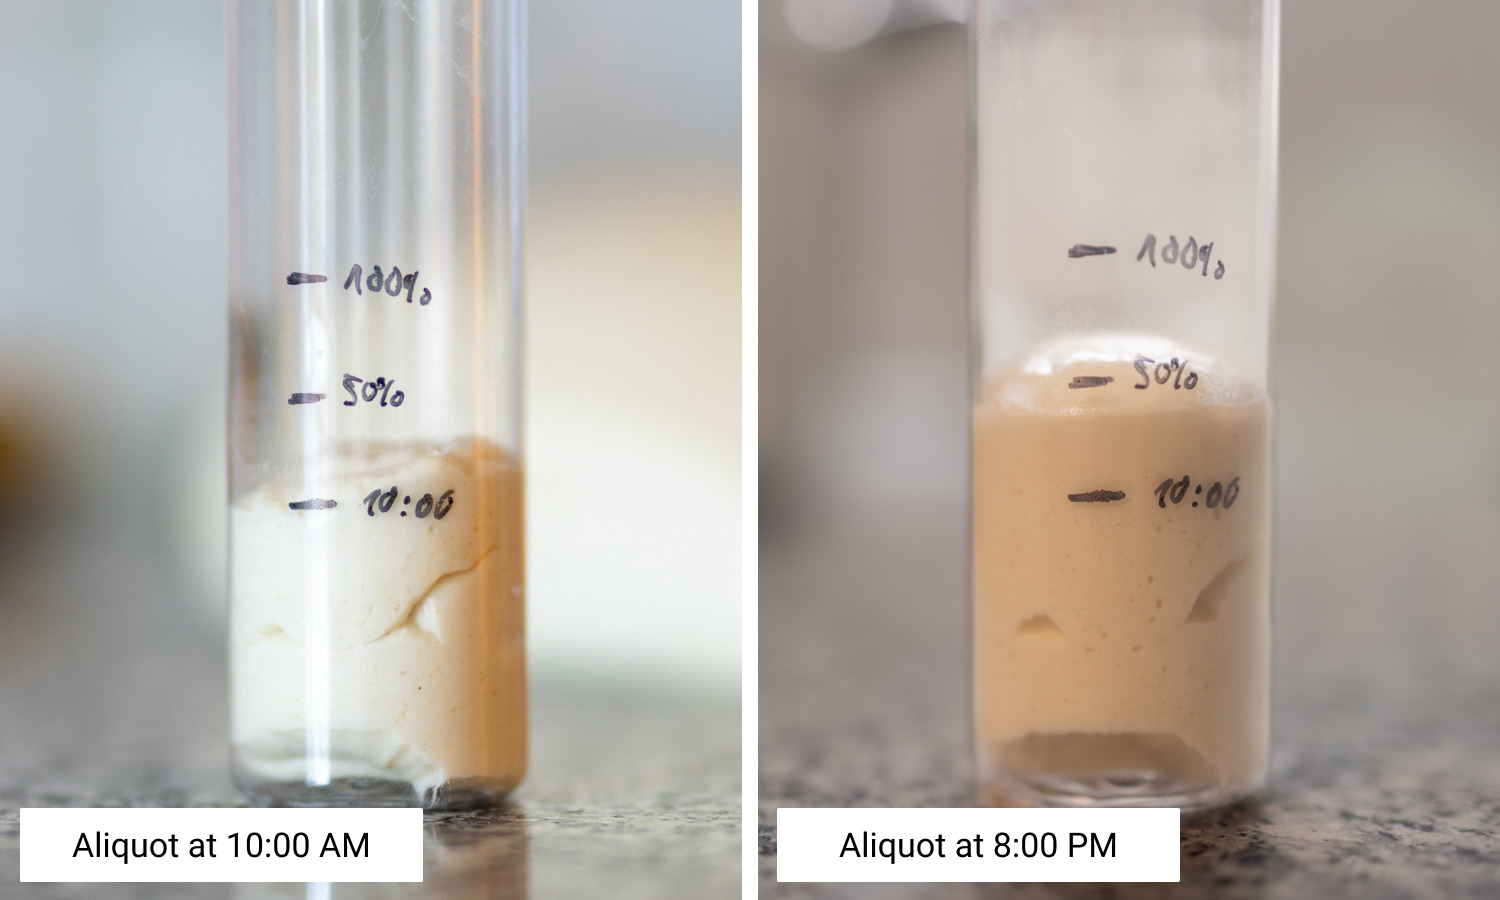
\includegraphics[width=\textwidth]{aliquot-before-after}
  \caption{An aliquot jar to monitor the dough's fermentation progress.
  It took 10 hours for the dough to reach a 50 percent size increase.}
\end{figure}

While the aliquot jar has enabled me to consistently bake
great loaves there are limitations to consider. It's crucial
to use a cylindrical-shaped container to properly judge
the dough's size increase. Furthermore, it is essential
to use room-temperature water when making your dough. If the
water is hotter, your aliquot due to its smaller size
will cool down faster. The aliquot will ferment slower
than your dough. Similarly, when you use too cold water,
your sample will heat up faster than the large dough mass.
In that case, your aliquot is ahead of your main dough. You
would probably stop the fermentation too early. Make sure
to keep the dough and aliquot close together. Some people even
place the aliquot in the same container. This makes sure that
both are in the same environment temperature. The aliquot
is also less reliable if your ambient temperature changes
a lot during the day. In that case, your aliquot will adapt
faster than your main dough. The readings will always be slightly
off. If you are making a large chunk of dough with more
than 10kg of flour the jar is also less reliable. The biochemical
reactions happening inside your dough will heat it.
The fermentation itself is exothermic which means
that it produces heat.

Another but more expensive option is to use a pH meter
to monitor your dough's fermentation state. As the lactic
and acetic acid bacteria ferment, more acidity is piled
up inside your dough. The acidity value (pH) can be
measured using such a meter. The more acidity the lower the pH
value of your dough. The pH scale is logarithmic meaning
that each digit change will have a 10x increase in acidity.
A sourdough dough might begin fermenting at a pH of 6,
then shortly before baking has a pH of around 4. This means
that the dough itself is 10x times 10x (= 100x) sourer
than at the beginning. By using the meter you can always
judge the state of your dough's acidification and then act
accordingly.

To use the pH meter successfully you need to find pH values
that work for your dough. Depending on your starter,
water, and flour composition the pH values to look out
for are different. A stronger flour with more gluten
can be fermented for a longer period. To find out
the pH values for your bread I recommend taking
several measurements while making your dough.

\begin{enumerate}
  \item Measure the pH value of your sourdough starter before using it
  \item Check the pH after mixing all the ingredients
  \item Check the pH before dividing and pre-shaping
  \item Check the pH before shaping
  \item Check the pH of your dough before and after proofing
  \item Check the pH of your bread after baking
\end{enumerate}

If the bread you made turned out successful with your values
you can use them as a reference for your next batch. If the
bread didn't turn out the way you like, either shorten
the fermentation or extend it a little bit.

\begin{table}[!htb]
  \begin{tabular}{|l|r|}
  \hline
  \textbf{Step}       & \multicolumn{1}{l|}{\textbf{pH Value}} \\ \hline
  Starter ready       & 4.20                                   \\ \hline
  Mixing              & 6.00                                   \\ \hline
  Dividing/preshaping & 4.10                                   \\ \hline
  Shaping             & 4.05                                   \\ \hline
  Before proofing     & 4.03                                   \\ \hline
  After proofing      & 3.80                                   \\ \hline
  After baking        & 3.90                                   \\ \hline
  \end{tabular}
  \caption{Example pH values for the different breakpoints of my own sourdough process}
  \label{table:sample-ph-values}
\end{table}

The beauty of this method is its reliability. Once you found
out your good working values, you can reproduce
the same level of fermentation with each subsequent dough.
This is especially handy for large-scale bakeries that want
to achieve consistency in each bread.

While this method is very reliable there are also certain
limitations to consider.

First of all the pH values that work for me likely won't work for
you. Depending on your own starter's composition of lactic 
and acetic acid bacteria your pH values will be different.
You can use the values shown in table \ref{table:sample-ph-values}
as rough ballpark figures. Regardless you need to find values
that work for your setup.

Another limitation is the price. You will need to purchase
a high-tech pH meter. Ideally, a meter featuring a spearhead.
This way you can directly poke the meter deep into the dough.
At the same time, automated temperature adjustments are a
feature to look out for. Depending on the temperature
the pH value varies. There are tables you can use to
do the adjustment calculations. More expensive meters
have this feature built-in. The pH meter loses accuracy
over time. For this reason, you need to frequently
calibrate this. The process is cumbersome and takes time.
Lastly, you need to carefully rinse the pH meter before
using it in your dough. The liquid surrounding the
head of your pH meter is not food-safe and thus should
not be eaten. I rinse the meter for at least one minute
before using it to measure my dough's fermentation stage.

The last method to judge the state of bulk fermentation
is to read the signs of your dough. The more bread you are
made the more accustomed you will become to this process.
Look out for the dough's size increase. This can sometimes
be a challenge when your dough is inside a container.
You can help yourself by marking your container. Some bakers
even use a transparent rectangular bulk container. You
can use a pen to mark the initial starting point. From there
on you can nicely observe the size increase. Similar to the
mentioned aliquot jar look out for a size increase that works
for your sourdough composition.

\begin{figure}[!htb]
  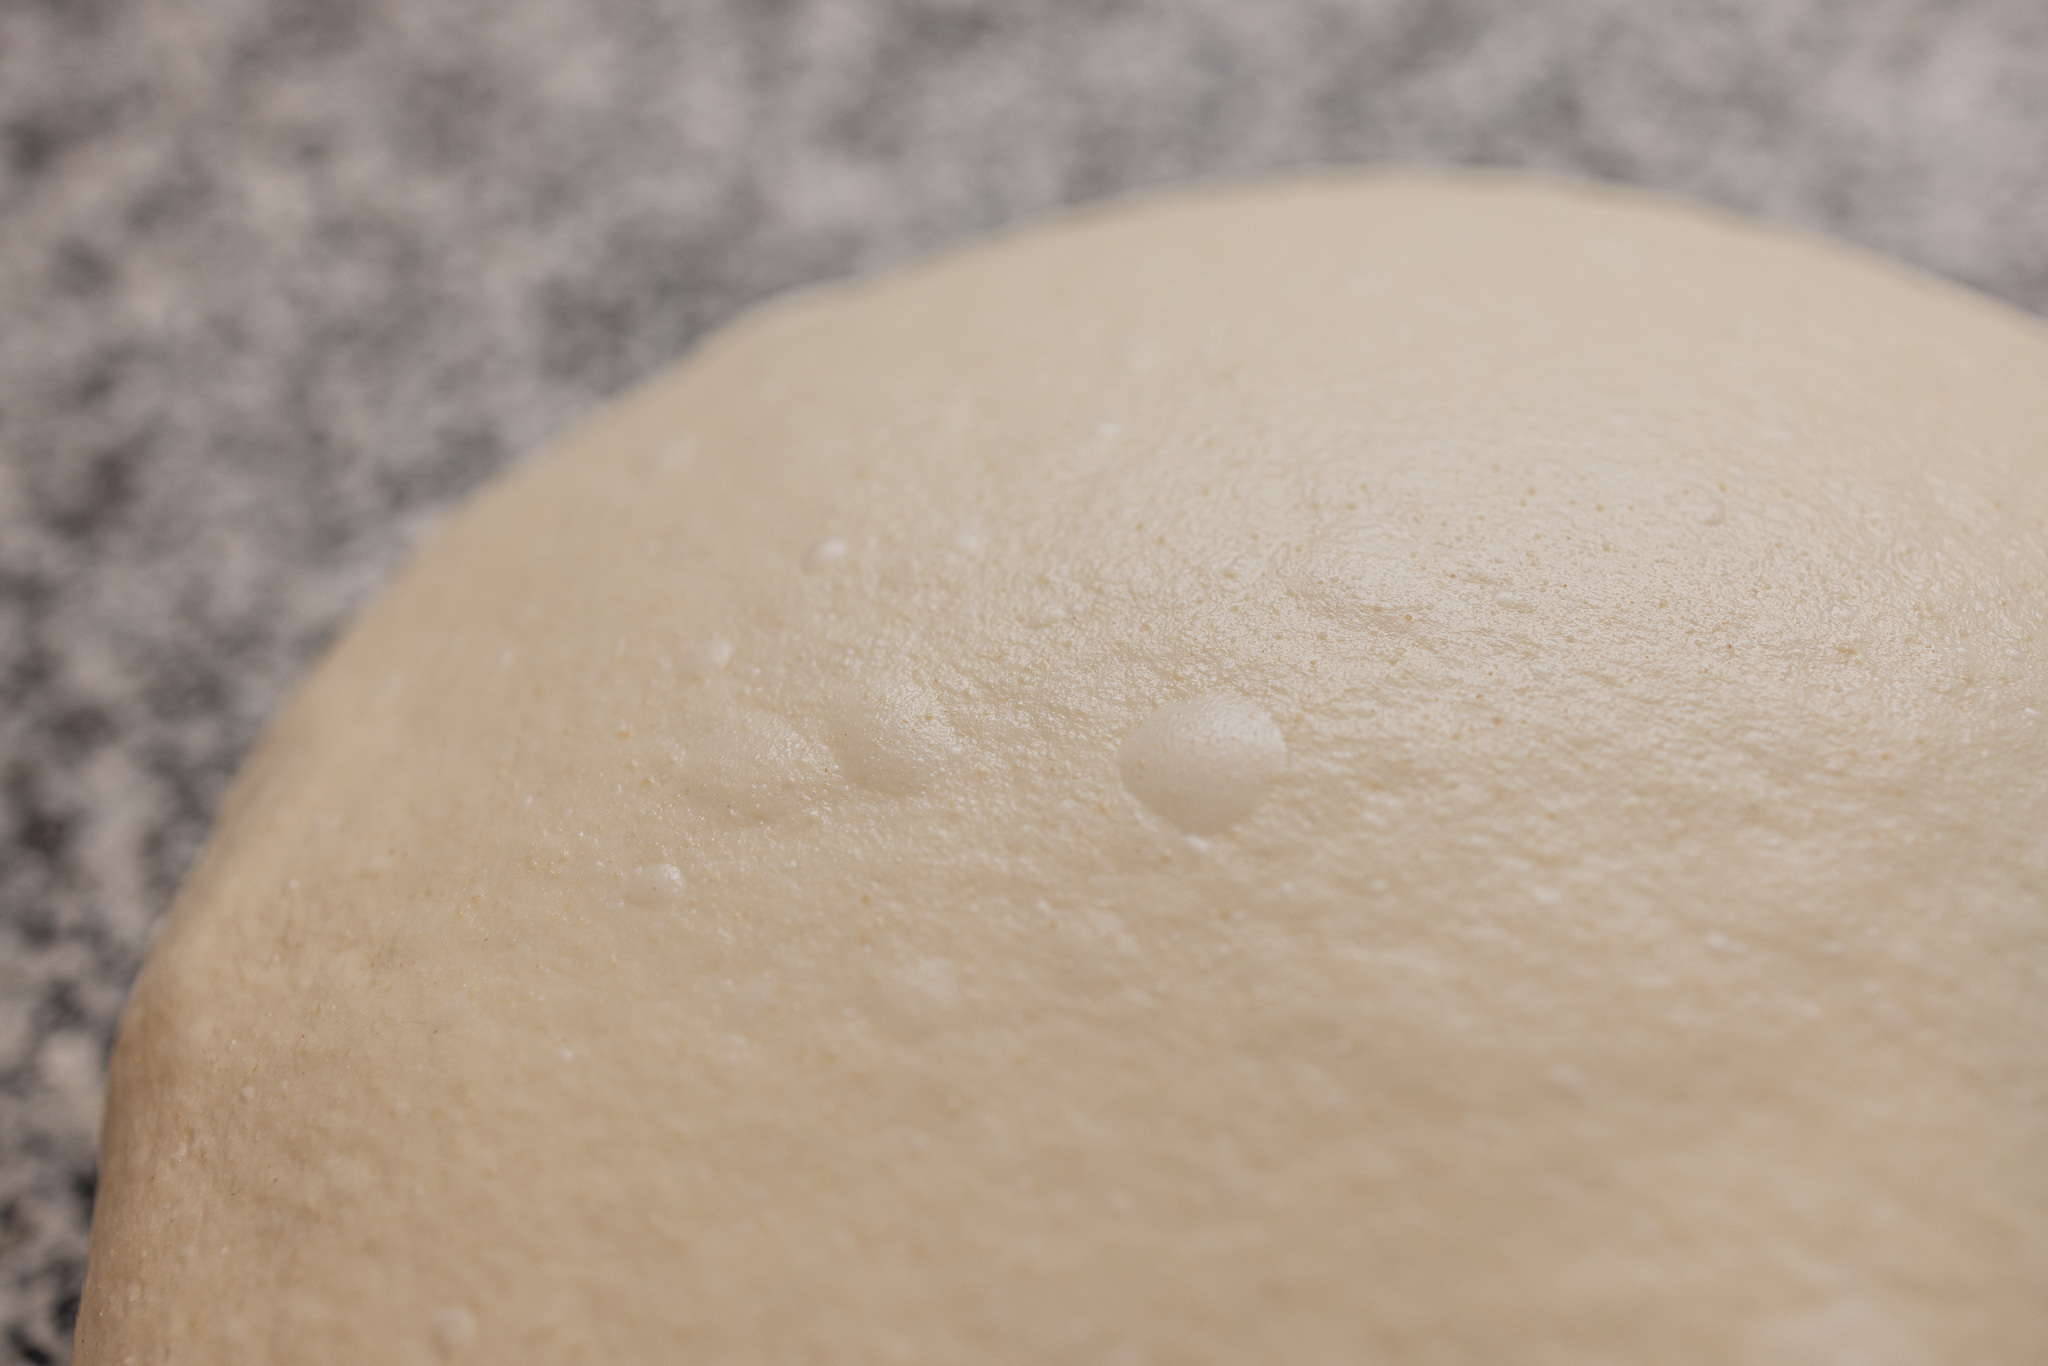
\includegraphics[width=\textwidth]{bulk-finished-dough}
  \caption{A dough in a good state to finish bulk fermentation. Notice
  the tiny bubbles on the dough's surface. They are a sign that the dough
  is inflated well enough.}
\end{figure}

Look out for bubbles on the surface of your dough. They
are a good sign that your dough is inflated with gas. The
further you push the bulk fermentation the more bubbles
will appear. If you overdo this stage the dough becomes leaky and
the bubbles will disappear again.

Take note of the dough's smell. It should match the same
smell of a ripe starter shortly before collapsing. As mentioned
before, your dough is nothing but a gigantic starter. You
can also proceed and taste your dough. It will taste like
pickled food. Depending on the acidity you can judge how
far the dough is in the fermentation process. The final bread
will taste less sour. That's because a lot of acid evaporates
during baking.\footnote{More on this topic later.
Just by baking longer and/or shorter, you can control
the tang of your final baked bread. The longer
you bake the less sour the final loaf. The shorter
the more acidity is still inside the bread. The resulting
loaf will be sourer.}

When touching the dough it should feel tacky
on your hands. The dough should also be less sticky
compared to earlier stages. If the dough is overly
sticky you have pushed the fermentation too far.

If you pushed the bulk fermentation too far you won't be able
to bake a free-standing loaf with the dough anymore. But don't
worry. You can move your dough into a loaf pan, or use parts
of the dough as the starter for your next dough. When using
a loaf pan make sure it's properly greased. You might have
to use a spatula to transfer your dough. Allow the dough
to proof for at least 30 minutes in the loaf pan before
baking it. This makes sure that large cavities induced
by the transfer are evened out. You could push the proofing
stage to 24 hours or even 72 hours. The resulting
bread would feature an excellent very tangy taste.


\section{Stretch and folds}
This chapter is still pending and will be added soon.

\section{Optional Preshaping}
This chapter is still pending and will be added soon.

\section{Shaping}
This chapter is still pending and will be added soon.

\section{Proofing}
This chapter is still pending and will be added soon.

\section{Scoring}
This chapter is still pending and will be added soon.
